\documentclass[11pt]{article}
\usepackage{graphicx}
\usepackage[section]{placeins}
\usepackage{amsmath}

\usepackage[top=1.0in, bottom=1.0in, left=0.5in, right=0.5in]{geometry}
\renewcommand{\thesection}{}
\renewcommand{\thesubsection}{\arabic{subsection}}

\begin{document}
\title{\vspace{15ex}\Huge{Physics Behind the Simulation: A CS296 Report by Group 12}\vspace{15ex}}


\author{
  Vikas Garg\\120050017\\
  \texttt{vikasgarg@iitb.ac.in}\\[1 cm]
  \and
  Ravi kumar Verma\\120050027\\
  \texttt{ravikumarverma1994@cse.iitb.ac.in}
  \and 
  Dheerendra Singh Rathor\\120050033\\
  \texttt{dheerendra@cse.iitb.ac.in}\\[1 cm]
}

\date{\today}
\maketitle
\newpage

\section{Introduction}
In our real life we interact with numourous physical bodies. Sometimes we know the physics behind them and sometimes not. Often we imagine someking of physical interaction in out mind and want to feel them. 
This report is about simulating physics on computer screen. We make our own physical world and want to see interaction in that world.physical world on the computer using Box2d\cite{Box2D} with the help of openGL in C++.


\section{Physics behind the simulation}
This contains contains the details about various  physical objects and their interaction in the Box2D simulation.
\subsection{Pendulam near the see-saw}
Pendulam is for controlling the velocity of the ball coming from the horizontal revolving bar and the final velocity of the ball is adjusted in a way such that it is exactly the same required for moving the light box to the open box in the end.
\begin{equation}
\begin{split}
\text{max angle of pendulam} = \arccos{\left( 1-\frac {v^2} {2gl} \right)}\cite{hcv}\\
\mathbf{v}=\text{velocity of ball } m/s\\
\mathbf{g}=\text{acceleration due to gravity } m/s^2\\
\mathbf{l}=\text{length of string of pendulam } m\\
\end{split}
\end{equation}
\begin{figure}[!ht]
\centering
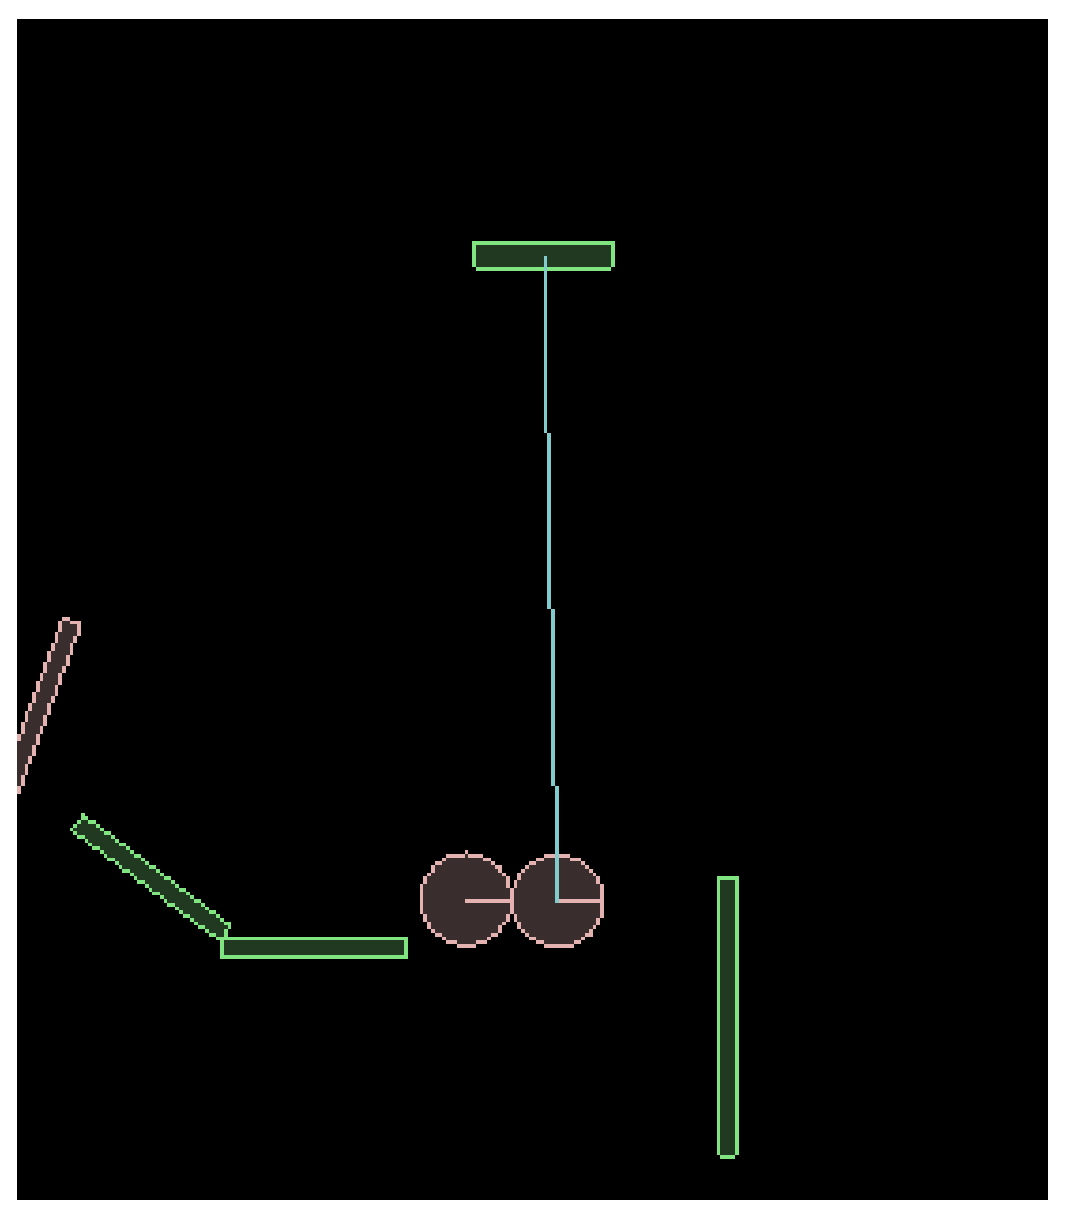
\includegraphics[scale=0.25]{pendulam}
\caption{This is working pendulam}
\label{fig1}
\end{figure}
\subsection{Ball on the top of the bar of pulley}
This ball is light ball and is kept on the top of the bar of the pulley. When the light box if jumped from see-saw, it reaches this
ball via above the bob of the pendulam in mentioned in above section. This box is triggered by that box and finally this rotates
the plank present below the pulley.
\begin{equation}
\begin{split}
\text{velocity of ball can be found by} \Rightarrow v_2 - v_1 = e\left( u_1 - u_2 \right) \\
\mathbf{v_2} : \text{velocity of ball after collision in } m/s\\
\mathbf{v_1} : \text{velocity of box after collision in } m/s\\
\mathbf{u_2} : \text{velocity of ball before collision in } m/s\\
\mathbf{u_1} : \text{velocity of box before collision in } m/s\\
\mathbf{e} : \text{coffiecient of restitution} \cite{rh}\\ 
\end{split}
\end{equation}
\begin{figure}[!ht]
\centering
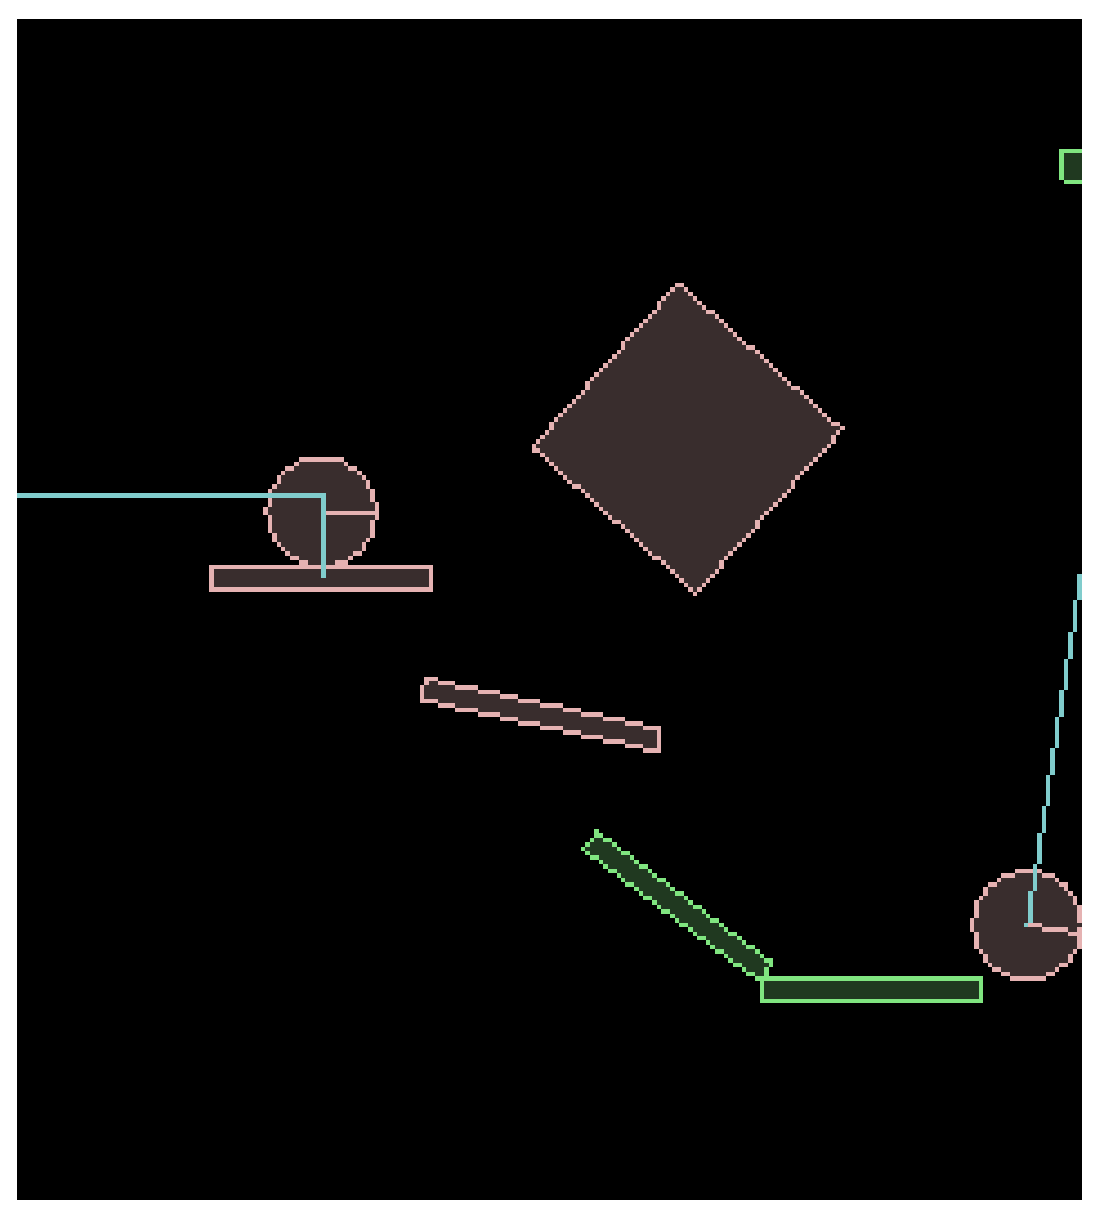
\includegraphics[scale=0.25]{ball_on_bar}
\caption{The ball above the bar of pulley}
\label{fig2}
\end{figure}
\subsection{Revolving plank \& ball below pulley}
This is the one of the finishing part of simulation. when the box hits the ball above the bar, that ball comes down to the revolving 
plank and ball which is supported by a stopper. The ball from the bar hits the ball here rotates the plank which give the light box an
option to slide down and end up in open box in left of the pulley
\begin{equation}
\begin{split}
\text{equation (2) is also require here due to collision}\\
\text{energy conservation} \Rightarrow \sum I \omega ^2= \mathbf{C} \\
\mathbf{I} : \text{Moment of Inertia } kg/m^2\\
\mathbf{\omega} : \text{ angular velocity } rad/s\\
\mathbf{C} : \text{Constant} \cite{flp}
\end{split}
\end{equation}
\begin{figure}[!ht]
\centering
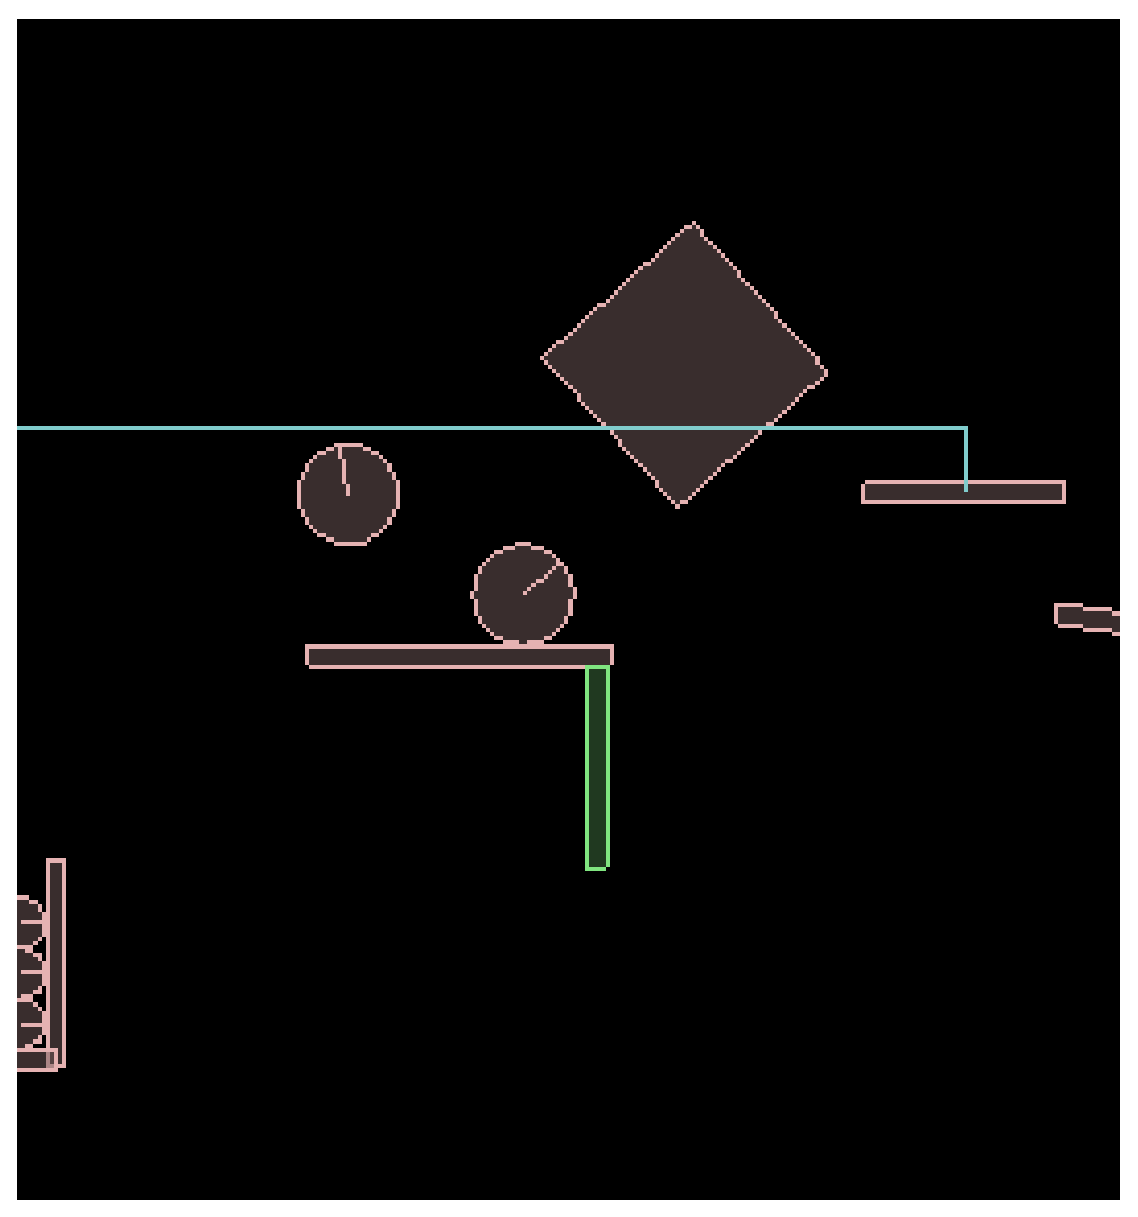
\includegraphics[scale=0.25]{revolve_platform}
\caption{The revolving platform and ball below the pulley}
\label{fig3}
\end{figure}
\section{Conclusions}
As we have seen, we have discussed a lot about simulation and equations used in them.
Here in Box2D simulation we had applied the physics to a virtual world and simulated them and 
have seen that virtual world is working exactly as formulated in the physics. And also we have seen
that Box2D is a great platform for simulating physics in 2-Dimensions.
\bibliographystyle{plain}
\bibliography{cs296_report_12}
\end{document}
